\documentclass[border=4pt,12pt]{standalone}
% House style for redrawn exam diagrams (diagram-v4: 0.4pt lines, filled -latex arrows, fine dashes; stipple and hatching drawn as real dots/lines (no PDF/SVG patterns, so they render in every browser and at any scale); transparent background). Every figure \input's this.
\usepackage{amsmath,amssymb}
\usepackage{txfonts}
\usepackage{pdfrender,xcolor}
% \halo{text}: label on shading. The shading stops just around each letter's outline (a thin knock-out that follows the
% glyphs, like the papers' typesetting), never a box. Owner: "I don't want a box around the text".
\newcommand{\halo}[1]{\leavevmode\rlap{\pdfrender{TextRenderingMode=2,LineWidth=2.2pt,LineJoinStyle=1,StrokeColor=white,FillColor=white}#1}#1}
\usepackage{tikz,pgfplots}
\pgfplotsset{compat=1.18}
\usetikzlibrary{arrows.meta,calc,angles,quotes,patterns,patterns.meta,intersections,positioning,decorations.markings,shapes.geometric}
% Stipple and hatching are drawn as actual dots / lines clipped to the region (path picture), NOT as pattern fills:
% SVG <pattern> fills vanish or blur when browsers scale the image, so the owner could not see the shading.
% Each dot is a 0.72pt square (keeps SVGs small; reads as a dot at print size). Dots sit on one global staggered grid, so neighbouring regions line up.
\makeatletter
\newdimen\ex@x \newdimen\ex@y \newdimen\ex@xa \newdimen\ex@ya \newdimen\ex@xb \newdimen\ex@yb \newcount\ex@row
\def\exam@stipplecolor{black!75}\def\exam@dotr{0.42pt}\def\exam@dotgap{2.5}
\def\ex@rowdots{\ifdim\ex@x<\ex@xb \pgfpathrectangle{\pgfqpoint{\dimexpr\ex@x-0.36pt\relax}{\dimexpr\ex@y-0.36pt\relax}}{\pgfqpoint{0.72pt}{0.72pt}}\advance\ex@x by \exam@dotgap pt\relax\expandafter\ex@rowdots\fi}
\def\exam@stipple{%
  \pgftransformreset% dots are sized in real points even inside scaled pictures
  \pgfpointanchor{path picture bounding box}{south west}\ex@xa=\pgf@x \ex@ya=\pgf@y
  \pgfpointanchor{path picture bounding box}{north east}\ex@xb=\pgf@x \ex@yb=\pgf@y
  \pgfsetfillcolor{\exam@stipplecolor}\pgfmathsetmacro\ex@h{\exam@dotgap/2}%
  \pgfmathtruncatemacro\ex@r{floor(\ex@ya/\ex@h)-1}\ex@row=\ex@r\relax
  \ex@y=\ex@r\dimexpr\ex@h pt\relax
  \loop\ifdim\ex@y<\ex@yb
    \pgfmathtruncatemacro\ex@c{floor(\ex@xa/\exam@dotgap)-1}\ex@x=\ex@c\dimexpr\exam@dotgap pt\relax
    \ifodd\ex@row \advance\ex@x by \ex@h pt\fi
    \ex@rowdots
    \advance\ex@y by \ex@h pt \advance\ex@row by 1
    \ifnum\numexpr\ex@row-(\ex@row/4)*4\relax=0 \pgfusepath{fill}\fi% flush every 4 rows: bounded TeX memory, few clip copies in the SVG
  \repeat\pgfusepath{fill}}
\newdimen\ex@d
\def\exam@hatch#1{% #1 = 1 for /, -1 for \ ; lines 45 degrees, 3pt apart
  \pgftransformreset
  \pgfpointanchor{path picture bounding box}{south west}\ex@xa=\pgf@x \ex@ya=\pgf@y
  \pgfpointanchor{path picture bounding box}{north east}\ex@xb=\pgf@x \ex@yb=\pgf@y
  \ex@d=\dimexpr\ex@yb-\ex@ya\relax \ex@x=\dimexpr\ex@xa-\ex@d\relax
  \loop\ifdim\ex@x<\ex@xb
    \ifnum#1>0 \pgfpathmoveto{\pgfqpoint{\ex@x}{\ex@ya}}\pgfpathlineto{\pgfqpoint{\dimexpr\ex@x+\ex@d\relax}{\ex@yb}}%
    \else \pgfpathmoveto{\pgfqpoint{\ex@x}{\ex@yb}}\pgfpathlineto{\pgfqpoint{\dimexpr\ex@x+\ex@d\relax}{\ex@ya}}\fi
    \advance\ex@x by 4.24pt
  \repeat
  \pgfsetlinewidth{0.4pt}\pgfsetstrokecolor{black}\pgfusepath{stroke}}
\def\examstipple{\exam@stipple}\def\examhatch{\exam@hatch}\def\examsetstipplecolor#1{\def\exam@stipplecolor{#1}}\def\examsetdotgap#1{\def\exam@dotgap{#1}}
\makeatother
% (legacy pattern kept for old files)
% staggered stipple like the NESA papers' dotted shading
\pgfdeclarepatternformonly{exam stipple}{\pgfpointorigin}{\pgfqpoint{2.2pt}{2.2pt}}{\pgfqpoint{2.2pt}{2.2pt}}{%
  \pgfpathcircle{\pgfqpoint{0.55pt}{0.55pt}}{0.42pt}\pgfpathcircle{\pgfqpoint{1.65pt}{1.65pt}}{0.42pt}\pgfusepath{fill}}
\tikzset{
  every picture/.style={line width=0.6pt, >={Latex[length=2mm,width=1.3mm]}},
  curve/.style={line width=0.6pt},
  open arrow/.style={-{Latex[length=2mm,width=1.3mm]}},  % owner: filled -latex heads everywhere, no open chevrons
  aux/.style={dash pattern=on 2pt off 1.5pt, line width=0.6pt},
  shade/.code={\def\exA{#1}\def\exB{none}\ifx\exA\exB\else\pgfkeysalso{fill=black!18}\fi},
  shade/.default=on,
  shade dots/.style={fill=none, path picture={\examstipple}},
  stipple color/.code={\examsetstipplecolor{#1}},
  stipple gap/.code={\examsetdotgap{#1}},
  shade dense dots/.style={fill=none, stipple gap=1.6, path picture={\examstipple}},
  shade hatch/.style={fill=none, path picture={\examhatch{1}}},
  shade hatch reverse/.style={fill=none, path picture={\examhatch{-1}}},
  shade solid/.style={fill=black},
  pt/.style={circle, fill, inner sep=1.1pt},
  open pt/.style={circle, draw, fill=white, inner sep=1.1pt},
}
\pgfplotsset{
  exam axes/.style={axis lines=middle, axis line style={->}, xlabel={$x$}, ylabel={$y$},
    xlabel style={anchor=west}, ylabel style={anchor=south}, tick label style={font=\small},
    every axis plot/.append style={line width=0.6pt, black}, samples=200, clip=false,
    enlargelimits=false, axis on top},
}

\begin{document}
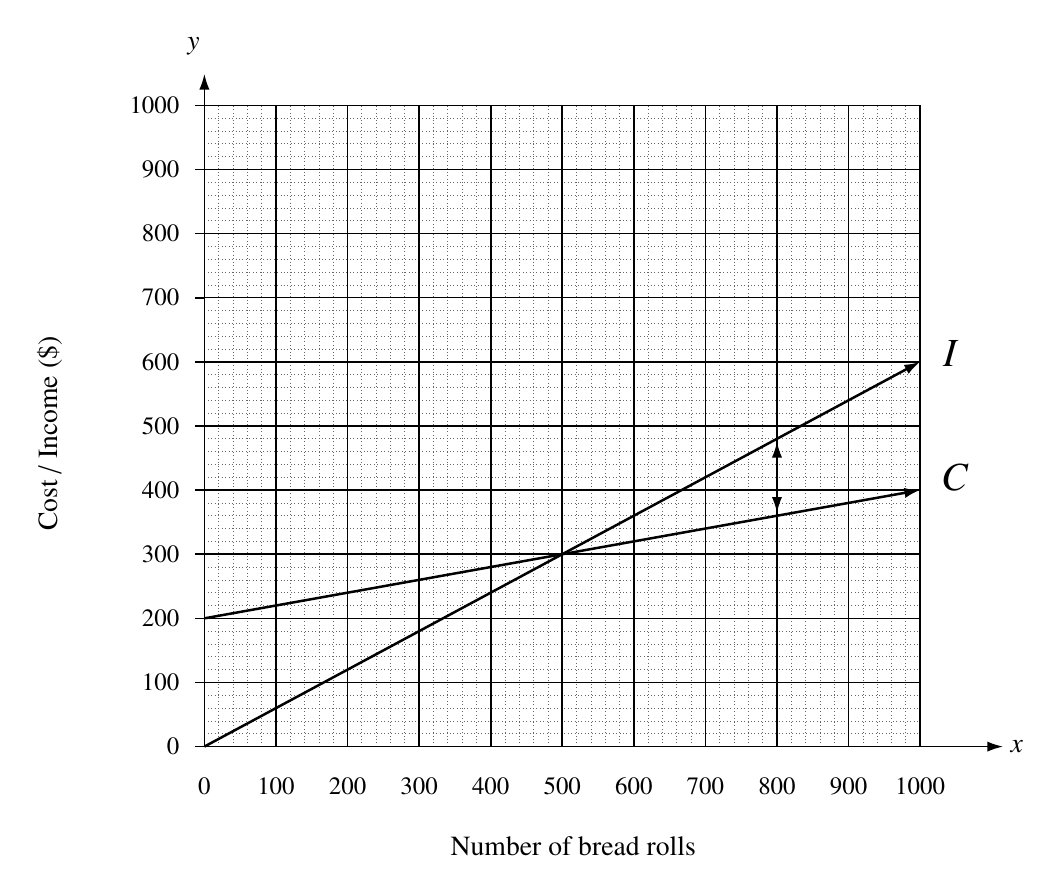
\begin{tikzpicture}[x=0.0127cm,y=-0.0127cm]
  % solution: C=200+0.2n and I=0.6n on the answer grid; break-even (500,300); profit $120 at n=800 (I-C=480-360)
  \draw[densely dotted, line width=0.25pt, black!60] (257.3,748.0) -- (257.3,106.5) (271.6,748.0) -- (271.6,106.5) (286.0,748.0) -- (286.0,106.5) (300.3,748.0) -- (300.3,106.5) (328.9,748.0) -- (328.9,106.5) (343.2,748.0) -- (343.2,106.5) (357.6,748.0) -- (357.6,106.5) (371.9,748.0) -- (371.9,106.5) (400.5,748.0) -- (400.5,106.5) (414.8,748.0) -- (414.8,106.5) (429.2,748.0) -- (429.2,106.5) (443.5,748.0) -- (443.5,106.5) (472.1,748.0) -- (472.1,106.5) (486.4,748.0) -- (486.4,106.5) (500.8,748.0) -- (500.8,106.5) (515.1,748.0) -- (515.1,106.5) (543.7,748.0) -- (543.7,106.5) (558.0,748.0) -- (558.0,106.5) (572.4,748.0) -- (572.4,106.5) (586.7,748.0) -- (586.7,106.5) (615.3,748.0) -- (615.3,106.5) (629.6,748.0) -- (629.6,106.5) (644.0,748.0) -- (644.0,106.5) (658.3,748.0) -- (658.3,106.5) (686.9,748.0) -- (686.9,106.5) (701.2,748.0) -- (701.2,106.5) (715.6,748.0) -- (715.6,106.5) (729.9,748.0) -- (729.9,106.5) (758.5,748.0) -- (758.5,106.5) (772.8,748.0) -- (772.8,106.5) (787.2,748.0) -- (787.2,106.5) (801.5,748.0) -- (801.5,106.5) (830.1,748.0) -- (830.1,106.5) (844.4,748.0) -- (844.4,106.5) (858.8,748.0) -- (858.8,106.5) (873.1,748.0) -- (873.1,106.5) (901.7,748.0) -- (901.7,106.5) (916.0,748.0) -- (916.0,106.5) (930.4,748.0) -- (930.4,106.5) (944.7,748.0) -- (944.7,106.5) (243.0,735.2) -- (959.0,735.2) (243.0,722.3) -- (959.0,722.3) (243.0,709.5) -- (959.0,709.5) (243.0,696.7) -- (959.0,696.7) (243.0,671.0) -- (959.0,671.0) (243.0,658.2) -- (959.0,658.2) (243.0,645.4) -- (959.0,645.4) (243.0,632.5) -- (959.0,632.5) (243.0,606.9) -- (959.0,606.9) (243.0,594.0) -- (959.0,594.0) (243.0,581.2) -- (959.0,581.2) (243.0,568.4) -- (959.0,568.4) (243.0,542.7) -- (959.0,542.7) (243.0,529.9) -- (959.0,529.9) (243.0,517.1) -- (959.0,517.1) (243.0,504.2) -- (959.0,504.2) (243.0,478.6) -- (959.0,478.6) (243.0,465.7) -- (959.0,465.7) (243.0,452.9) -- (959.0,452.9) (243.0,440.1) -- (959.0,440.1) (243.0,414.4) -- (959.0,414.4) (243.0,401.6) -- (959.0,401.6) (243.0,388.8) -- (959.0,388.8) (243.0,375.9) -- (959.0,375.9) (243.0,350.3) -- (959.0,350.3) (243.0,337.4) -- (959.0,337.4) (243.0,324.6) -- (959.0,324.6) (243.0,311.8) -- (959.0,311.8) (243.0,286.1) -- (959.0,286.1) (243.0,273.3) -- (959.0,273.3) (243.0,260.5) -- (959.0,260.5) (243.0,247.6) -- (959.0,247.6) (243.0,222.0) -- (959.0,222.0) (243.0,209.1) -- (959.0,209.1) (243.0,196.3) -- (959.0,196.3) (243.0,183.5) -- (959.0,183.5) (243.0,157.8) -- (959.0,157.8) (243.0,145.0) -- (959.0,145.0) (243.0,132.2) -- (959.0,132.2) (243.0,119.3) -- (959.0,119.3);
  \draw (314.6,748.0) -- (314.6,106.5) (386.2,748.0) -- (386.2,106.5) (457.8,748.0) -- (457.8,106.5) (529.4,748.0) -- (529.4,106.5) (601.0,748.0) -- (601.0,106.5) (672.6,748.0) -- (672.6,106.5) (744.2,748.0) -- (744.2,106.5) (815.8,748.0) -- (815.8,106.5) (887.4,748.0) -- (887.4,106.5) (959.0,748.0) -- (959.0,106.5) (243.0,683.9) -- (959.0,683.9) (243.0,619.7) -- (959.0,619.7) (243.0,555.5) -- (959.0,555.5) (243.0,491.4) -- (959.0,491.4) (243.0,427.2) -- (959.0,427.2) (243.0,363.1) -- (959.0,363.1) (243.0,298.9) -- (959.0,298.9) (243.0,234.8) -- (959.0,234.8) (243.0,170.6) -- (959.0,170.6) (243.0,106.5) -- (959.0,106.5);
  \draw[->] (243,748) -- (1042,748);
  \draw[->] (243,748) -- (243,75);
  \foreach \v in {0,...,10} \draw (234,{748-64.15*\v}) -- (243,{748-64.15*\v});
  \node[font=\small] at (243.0,788) {$0$};
  \node[font=\small] at (314.6,788) {$100$};
  \node[font=\small] at (386.2,788) {$200$};
  \node[font=\small] at (457.8,788) {$300$};
  \node[font=\small] at (529.4,788) {$400$};
  \node[font=\small] at (601.0,788) {$500$};
  \node[font=\small] at (672.6,788) {$600$};
  \node[font=\small] at (744.2,788) {$700$};
  \node[font=\small] at (815.8,788) {$800$};
  \node[font=\small] at (887.4,788) {$900$};
  \node[font=\small] at (959.0,788) {$1000$};
  \node[left,font=\small] at (228,748.0) {$0$};
  \node[left,font=\small] at (228,683.9) {$100$};
  \node[left,font=\small] at (228,619.7) {$200$};
  \node[left,font=\small] at (228,555.5) {$300$};
  \node[left,font=\small] at (228,491.4) {$400$};
  \node[left,font=\small] at (228,427.2) {$500$};
  \node[left,font=\small] at (228,363.1) {$600$};
  \node[left,font=\small] at (228,299.0) {$700$};
  \node[left,font=\small] at (228,234.8) {$800$};
  \node[left,font=\small] at (228,170.7) {$900$};
  \node[left,font=\small] at (228,106.5) {$1000$};
  \node at (232,47) {$y$};
  \node at (1055,748) {$x$};
  \node at (612,848) {Number of bread rolls};
  \node[rotate=90] at (88,435) {Cost / Income (\$)};
  \draw[->,line width=0.9pt] (243.0,619.7) -- (959.0,491.4);
  \draw[->,line width=0.9pt] (243.0,748.0) -- (959.0,363.1);
  \node[font=\Large,right] at (971.0,355.1) {$I$};
  \node[font=\Large,right] at (971.0,479.4) {$C$};
  \draw[<->] (815.8,514.1) -- (815.8,443.1);
\end{tikzpicture}
\end{document}
